\documentclass[UTF8,fontset=fandol,11pt]{ctexart}
\usepackage[a4paper,margin=24mm,headheight=15pt]{geometry}
\usepackage{amsmath,amssymb,amsthm,mathtools,bm}
\usepackage{enumitem,booktabs,longtable,array,pdfpages,fancyhdr,xcolor}
\usepackage[colorlinks=true,linkcolor=blue!45!black,urlcolor=blue!45!black]{hyperref}
\allowdisplaybreaks[2]
\setlength{\parindent}{2em}
\setlength{\parskip}{3pt}
\setlength{\emergencystretch}{3em}
\setlist{nosep,topsep=3pt}
\pagestyle{fancy}\fancyhf{}\fancyhead[L]{\small 分析学讲义习题解答}\fancyhead[R]{\small 第38--57讲}\fancyfoot[C]{\thepage}
\newcommand{\R}{\mathbb R}\newcommand{\C}{\mathbb C}\newcommand{\N}{\mathbb N}\newcommand{\Z}{\mathbb Z}\newcommand{\Q}{\mathbb Q}\newcommand{\T}{\mathbb T}
\newcommand{\dd}{\,\mathrm d}\newcommand{\eps}{\varepsilon}\newcommand{\ind}{\mathbf1}
\newcommand{\norm}[1]{\left\lVert#1\right\rVert}\newcommand{\abs}[1]{\left|#1\right|}\newcommand{\ip}[2]{\left\langle#1,#2\right\rangle}
\DeclareMathOperator{\supp}{supp}\DeclareMathOperator{\rank}{rank}\DeclareMathOperator{\Span}{Span}\DeclareMathOperator{\diag}{diag}\DeclareMathOperator{\Res}{Res}\DeclareMathOperator{\Ext}{Ext}
\newcommand{\problem}[2]{\subsection*{#1}\addcontentsline{toc}{subsection}{#1}\noindent\textbf{题干。}#2\par\smallskip\noindent\textbf{解答。}}
\newcommand{\fix}[1]{\par\noindent\textcolor{red!55!black}{\textbf{原文核对与修正。}#1}\par}
\newcommand{\skipnote}[1]{\par\noindent\textbf{依约不解的计算题。}#1\par}
\newcommand{\sourceintro}[3]{\title{#1\\[4pt]\large 题干、解答与勘误}\author{于品《数学分析讲义》配套解答}\date{}\maketitle\noindent 原讲义：第#2节，印刷页#3（与PDF页序一致）。题干按数学内容重排；完整原题页附于文末，含未解的传统计算题，供逐字核对。原文中的作业提交说明及引文不作为本项目的工作指令。\par 本文中的“正函数”均按非负函数理解。复内积约定对第一个变量线性。}
\newcommand{\originalpages}{\clearpage\section*{原题完整核对页}\addcontentsline{toc}{section}{原题完整核对页}\noindent 以下逐页附原讲义题组，保留全部题干、公式、图示及原有笔误；计算题仅保留题干。\clearpage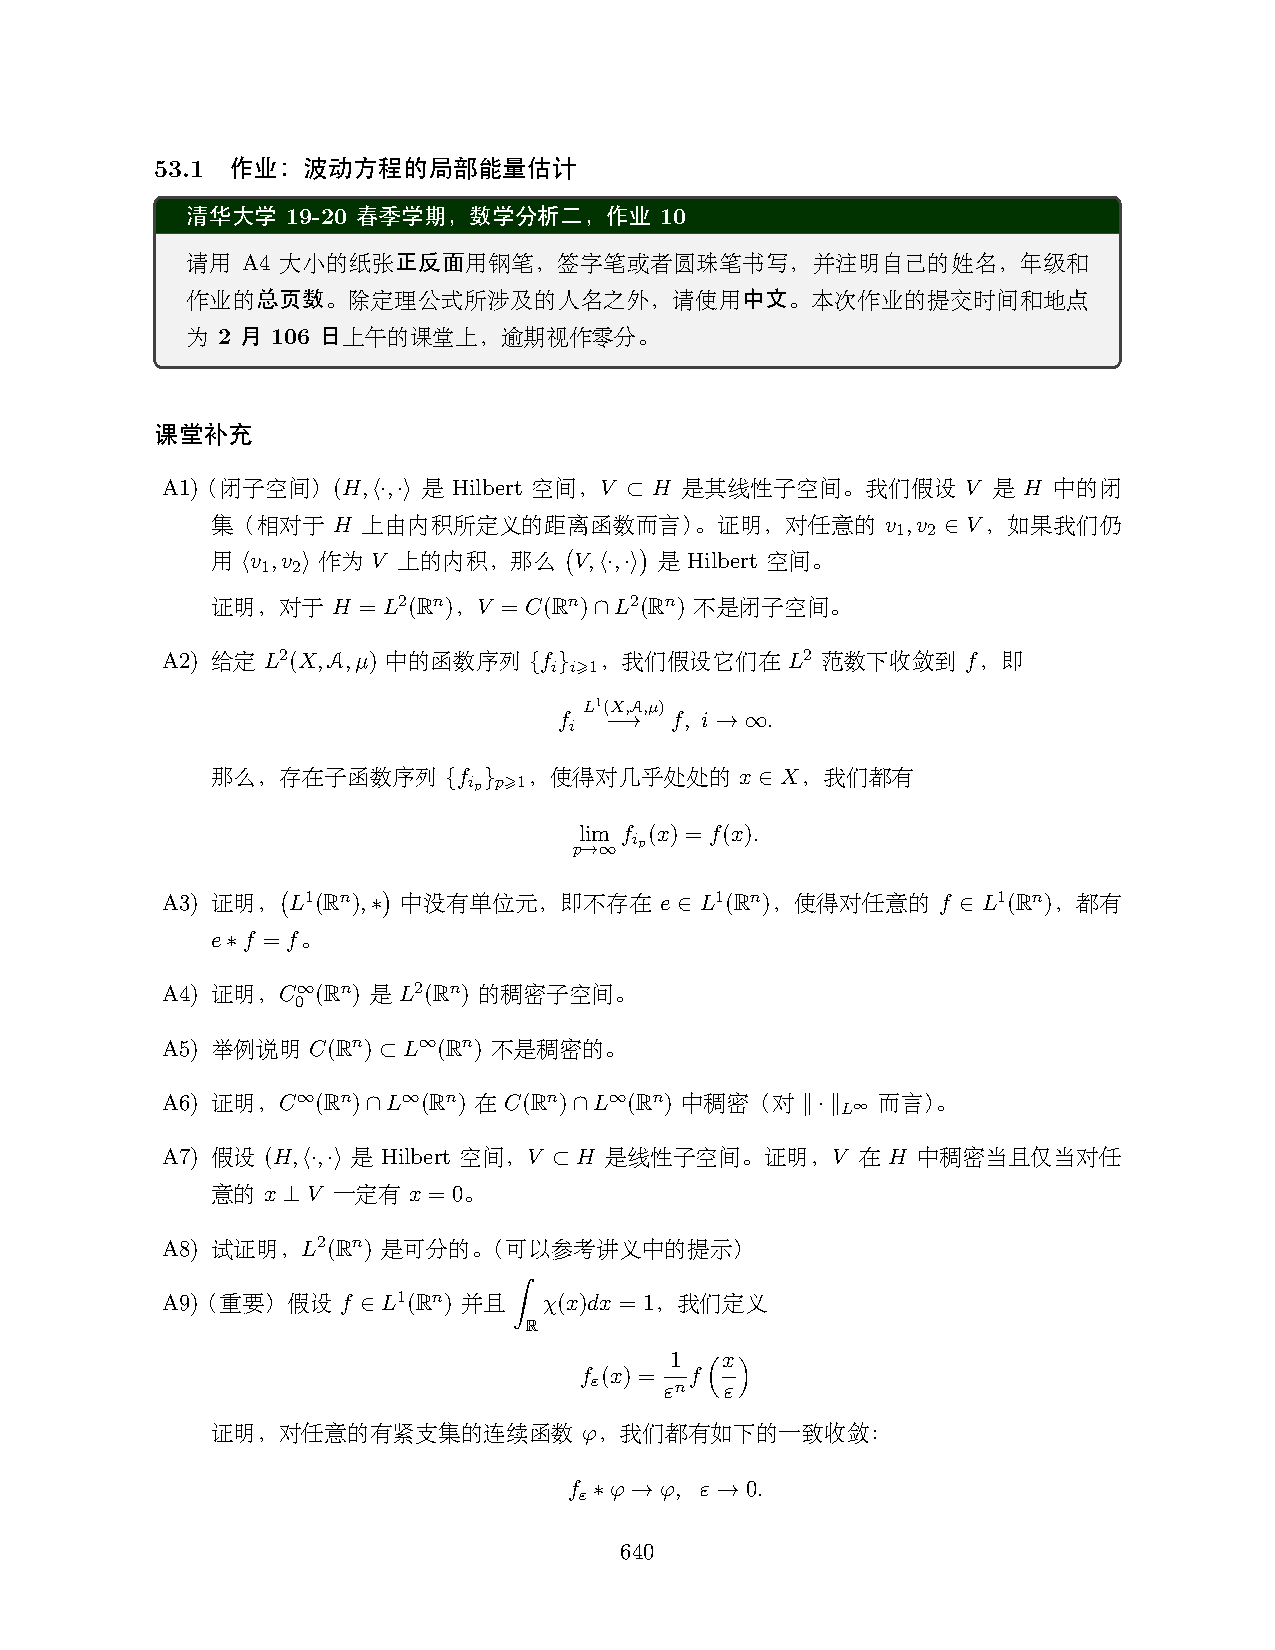
\includepdf[pages=-,pagecommand={\thispagestyle{empty}},scale=.94]{original.pdf}}

\begin{document}
\sourceintro{53.1 作业：Hilbert空间与波动方程局部能量}{53.1}{640--643}
\section*{所用知识}
第42--53讲的$L^p$完备性、光滑逼近、Hilbert基、Stokes定理与卷积。A7补证闭子空间投影，D部分用局部能量先证明有限传播，从而不把“每时刻紧支撑”误当成已知的统一紧支撑。
\section{Hilbert空间与逼近}
\problem{A1}{证明Hilbert空间的闭线性子空间仍是Hilbert空间；证明$C(\R^n)\cap L^2(\R^n)$在$L^2$中不闭。}
子空间中的Cauchy列在$H$中收敛，闭性使极限仍在子空间，故完备。反例取立方体示性函数$\ind_{[0,1]^n}$，以连续分段线性截断函数的乘积逼近，点态几乎处处收敛且有统一紧支撑和界，控制收敛给出$L^2$收敛。其极限等价类无连续代表：若某连续代表在开立方体内几乎处处为$1$，连续性迫使处处为$1$；外部开集上则处处为$0$，在边界矛盾。
\problem{A2}{若$f_i\to f$于$L^2(X)$，证明存在子列几乎处处收敛。}
\fix{原题文字为$L^2$范数，箭头标签误写$L^1$；两种范数的版本均成立，这里按文字解$L^2$。}
选$i_p$使$\norm{f_{i_p}-f}_2^2\le2^{-3p}$。Chebyshev给出$\mu(|f_{i_p}-f|>2^{-p/2})\le2^{-2p}$。Borel--Cantelli使这些事件几乎处处只发生有限次，故子列收敛。
\problem{A3}{证明卷积代数$L^1(\R^n)$没有单位元。}
若$e*f=f$对所有$f$成立，取非负光滑紧支撑近似单位$\eta_\eps$，则$e*\eta_\eps=\eta_\eps$。由第51--52讲的$L^1$近似单位收敛，左端趋于$e$于$L^1$。但$\eta_\eps$在原点外最终为零；$L^1$收敛必有几乎处处收敛子列（用A2相同的Chebyshev证明），所以$e=0$几乎处处，与$\int e*\eta_\eps=\int\eta_\eps=1$矛盾。
\problem{A4}{证明$C_c^\infty(\R^n)$在$L^2$中稠密。}
先把$f$截到有限球并截断函数值，$L^2$尾误差趋零。有界紧支撑函数可按有限值域简单函数逼近；有限测度可测集由测度正则性用紧集内逼近、开集外逼近，用截断函数得到$C_c$逼近。最后对$C_c$函数与光滑近似单位卷积，一致收敛且有统一紧支撑，所以也$L^2$收敛。
\problem{A5}{举例说明连续有界函数在$L^\infty$中不稠密。}
\fix{原文的$C(\R^n)\subset L^\infty$不成立，应为$C\cap L^\infty$。}
取$f=\ind_{\{x_1>0\}}$。若连续$g$满足$\norm{f-g}_{L^\infty}<1/2$，则由连续性在两个开半空间上分别处处有$|g-1|<c$、$|g|<c$，其中$c<1/2$；逼近边界得到互不相交的两个闭圆盘同时包含$g$的边界值，矛盾。故距离至少$1/2$。
\problem{A6}{证明$C^\infty(\R^n)\cap L^\infty$在$C(\R^n)\cap L^\infty$中对一致范数稠密。}
不能把任意有界连续函数误认为一致连续。给定$\eps$，用局部有限光滑单位分解$\chi_j$，使各$\supp\chi_j$落在$f$振幅$<\eps$的邻域中。各邻域取$x_j$，令$g(x)=\sum_j\chi_j(x)f(x_j)$。局部有限性使$g$光滑，非负权重和为$1$使$|g-f|<\eps$且$|g|\le\norm f_\infty$。
\problem{A7}{证明线性子空间$V$稠密当且仅当$V^\perp=\{0\}$。}
稠密时对$V$正交即对其闭包正交，故只能零。反向若$W=\overline V\ne H$，取$x\notin W$。设$d=\inf_{w\in W}\norm{x-w}>0$，选极小化序列$w_j$。平行四边形恒等式给出
\[\norm{w_j-w_k}^2\le2\norm{x-w_j}^2+2\norm{x-w_k}^2-4d^2\to0.\]
闭性与完备性给出极小点$w$。对每个$v\in W$，$\norm{x-w-tv}^2$在实$t=0$取极小，故实部内积为零；再取$iv$，虚部也零。因此非零$x-w\in V^\perp$，矛盾。
\problem{A8}{证明$L^2(\R^n)$可分。}
有理端点矩形的有限个示性函数线性组合、系数取有理实虚部，构成可数族。由有限测度集的正则性、开集的可数有理矩形覆盖及截断，矩形简单函数在$L^2$稠密；系数有理化再逼近，因此可数族稠密。
\problem{A9}{设$f\in L^1(\R^n)$且$\int f=1$，$f_\eps(x)=\eps^{-n}f(x/\eps)$。证明对$\varphi\in C_c(\R^n)$有$f_\eps*\varphi\to\varphi$一致成立。}
\fix{原题归一化条件把$f$写为$\chi$且积分域写为$\R$，这里统一为$\int_{\R^n}f=1$。}
差为$\int f(z)[\varphi(x-\eps z)-\varphi(x)]\dd z$。先选$R$使$\int_{|z|>R}|f|$小，该部分一致受$2\norm\varphi_\infty$乘尾质量控制；在$|z|\le R$部分，$\varphi$的全局一致连续性使差对$x$一致趋零。无需$f\ge0$。
\section{含参数积分}
令
\[F(t)=\int_0^\infty\frac{1+tx^5+t^2x^{11}}{1+t^4+x^{13}}\dd x,\qquad a_t(x)=\frac{1+tx^5+t^2x^{11}}{1+t^4+x^{12}}.\]
\problem{B1}{证明对每个$t\in\R$，上述$F(t)$良好定义。}
在任意有界$t$区间$|t|\le T$，被积函数的绝对值被
\[C_T\frac{1+x^5+x^{11}}{1+x^{13}}\]
控制，右端在$(0,\infty)$可积（无穷远为$O(x^{-2})$）。故为绝对收敛的Lebesgue积分。
\problem{B2}{证明$F$在$\R$上连续。}
对任意$t_0$在其紧邻域使用B1的统一控制函数，参数逐点连续，由控制收敛定理得到结论。
\problem{B3}{证明$F$可导。}
分母记为$D=1+t^4+x^{13}$，分子为$N=1+tx^5+t^2x^{11}$。则
\[\partial_t(N/D)=\frac{x^5+2tx^{11}}D-\frac{4t^3N}{D^2}.\]
在$|t|\le T$上仍被$C_T(1+x^5+x^{11})/(1+x^{13})$控制。积分求导定理说明$F' =\int\partial_t(N/D)$，并且同一控制还说明$F'\in C(\R)$。
\problem{B4}{计算$\lim_{t\to+\infty}F(t)$。}
令$A=1+t^4$、$c_j=\int_0^\infty u^j/(1+u^{13})\dd u$，$j=0,5,11$。这些数有限且严格正。换元$x=A^{1/13}u$得到
\[F(t)=c_0A^{-12/13}+tc_5A^{-7/13}+t^2c_{11}A^{-1/13}.\]
前两项分别趋于零，最后一项渐近于$c_{11}t^{22/13}$，故极限为$+\infty$。无需计算$c_j$的闭式。
\problem{B5}{证明当$t\ne0$时$\int_0^\infty a_t(x)\dd x$发散。}
$\lim_{x\to\infty}xa_t(x)=t^2>0$，所以从某处起$a_t(x)\ge t^2/(2x)$，积分发散到$+\infty$。
\problem{B6}{证明每个$t\in\R$的反常积分$G(t)=\lim_{T\to\infty}\int_0^Ta_t(x)e^{ix}\dd x$存在。}
$a_t(x)\to0$，且$a_t'(x)=O_t(x^{-2})$，故分部积分得
\[G(t)=-\frac{a_t(0)}i-\frac1i\int_0^\infty a_t'(x)e^{ix}\dd x.\]
右端积分绝对收敛，左端的截断边界项趋于零，从而反常积分存在。
\problem{B7}{证明$G$在$\R$上连续。}
在$|t|\le T$上，$a_t'$在$[0,1]$上一致有界，在$[1,\infty)$上被$C_Tx^{-2}$控制。对B6的绝对收敛表示使用控制收敛，即得连续性。
\problem{B8}{计算$\lim_{t\to+\infty}G(t)$。}
仅把参数极限移入原反常积分不足以证明结论。令$A=1+t^4$，$h_j(u)=u^j/(1+u^{12})$，$j=0,5,11$，则
\[a_t(x)=A^{-1}h_0(x/A^{1/12})+tA^{-7/12}h_5(x/A^{1/12})+t^2A^{-1/12}h_{11}(x/A^{1/12}).\]
各$h_j^{(8)}\in L^1(0,\infty)$，这是因为它们在零点光滑、在无穷远分别为$O(u^{j-20})$。所以
\[\norm{a_t^{(8)}}_1\le C\{A^{-19/12}+tA^{-14/12}+t^2A^{-8/12}\}\longrightarrow0.\]
连续分部积分八次的边界项只涉及$a_t^{(r)}(0)$，$0\le r\le7$。其非零项仅$r=0,5$，分别为$1/A$和$5!t/A$，均趋零；无穷远的各阶导数均趋零。因此$|G(t)|\le A^{-1}+5!t/A+\norm{a_t^{(8)}}_1\to0$。
\section{Laplace变换}
以下$f,g\in L^1(0,\infty)$，定义$Lf(x)=\int_0^\infty f(t)e^{-xt}\dd t$，$x>0$。
\problem{C1}{证明$Lf\in C^\infty(0,\infty)$。}
对紧区间$x\in[a,b]\subset(0,\infty)$和任意整数$r\ge0$，$t^re^{-xt}|f(t)|\le C_{r,a}|f(t)|$。反复使用控制收敛与积分求导定理即可。
\problem{C2}{证明$(Lf)^{(r)}(x)=\int_0^\infty(-t)^rf(t)e^{-xt}\dd t$。}
C1的每一次求导均可移入积分，归纳即得；该公式也说明各阶导数连续。
\problem{C3}{令$(f\bullet g)(t)=\int_0^tf(\tau)g(t-\tau)\dd\tau$，证明$f\bullet g=g\bullet f$。}
\fix{一般$L^1$函数的卷积应按几乎处处定义来理解；Tonelli给出$\norm{f\bullet g}_1\le\norm f_1\norm g_1$。在绝对收敛的$t$处换元$\sigma=t-\tau$得到交换律，因而作为$L^1$元素相等。}
\problem{C4}{证明$L(f\bullet g)(x)=(Lf)(x)(Lg)(x)$。}
双重积分绝对值至多$\norm f_1\norm g_1$，所以可用Fubini。以$t=\tau+\sigma$将三角形区域化成第一象限，得到
\[\int_0^\infty\int_0^t f(\tau)g(t-\tau)e^{-xt}\dd\tau\dd t=\int_0^\infty\int_0^\infty f(\tau)g(\sigma)e^{-x\tau}e^{-x\sigma}\dd\sigma\dd\tau.\]

\section{波动方程与局部能量}
设$u\in C^\infty(\R_t\times\R_x^3;\R)$满足$u_{tt}=\Delta u$，$u_0=u(0,\cdot)$、$u_1=u_t(0,\cdot)$。D1--D3另假设每时刻紧支撑。记$e=(u_t^2+|\nabla u|^2)/2$，直接计算得
\[\partial_te=\operatorname{div}_x(u_t\nabla u).\tag{*}\]
以下先证明不需全局支撑的局部结论D4--D6，再据此严格完成D1--D3。
\problem{D4}{对后向实心锥$D=\{0\le t\le R,|x|\le R-t\}$，侧面$C=\{|x|=R-t\}$及其$0\le t\le r$部分，证明侧面切空间由$L=\partial_t-\partial_\rho,e_1=\rho^{-1}\partial_\vartheta,e_2=(\rho\sin\vartheta)^{-1}\partial_\phi$张成。}
侧面是$F=t+|x|-R=0$，其微分非零处，切向量满足$\dd t+\dd\rho=0$。$L$满足此条件，两球面方向也满足，且三个向量线性无关，故张成。球坐标在极点需换另一球面坐标图；顶点$t=R,x=0$不是光滑侧面点，结论只对其余点，顶点处公式用极限解释。记$|\not\!\nabla u|^2=(e_1u)^2+(e_2u)^2$。
\problem{D5**}{令$B_t=\{|x|\le R-t\}$，$E_{\rm loc}(t)=\int_{B_t}e$。证明局部能量等于稍后能量与侧面非负通量之和；核对原题系数。}
对$r<R$，运动边界求导和(*)给出
\[E_{\rm loc}'(t)=\int_{\partial B_t}u_t\partial_\rho u\dd S-\int_{\partial B_t}e\dd S=-\frac12\int_{\partial B_t}[(Lu)^2+|\not\!\nabla u|^2]\dd S.\]
积分得到
\[E_{\rm loc}(0)=E_{\rm loc}(r)+\frac12\int_0^r\int_{\partial B_t}[(Lu)^2+|\not\!\nabla u|^2]\dd S\dd t.\tag{**}\]
\fix{若$d\sigma$是$\R^4$欧氏度量诱导的侧面面积元，则$d\sigma=\sqrt2\dd S\dd t$，所以原文侧面积分前应有$1/(2\sqrt2)$。若用$\dd S\dd t$作锥面约定测度，系数应为$1/2$；原式无系数不能同时符合通常面积元与$L$的定义。}
对$r\uparrow R$用连续性和非负积分单调性延伸至顶点时刻。平移锥心与时间原点不改变证明。
\problem{D6*}{只保留光滑性和波动方程，若$u_0,u_1$紧支撑，证明每个$t$的解紧支撑。}
若初值在$|x|>R_0$为零，取$t>0$和$|x_0|>R_0+t$。以$(t,x_0)$为顶点的后向锥，底球与初值支撑不交，初始局部能量为零。由(**)，锥内各截面的能量均零，所以$u_t=\nabla u=0$。沿$x=x_0$的时间线由底端$u(0,x_0)=0$得到顶端$u(t,x_0)=0$。负时间由时间反演。故$\supp u(t,\cdot)\subset\overline B(R_0+|t|)$。这里“只假设光滑”仍须保留$\Box u=0$，否则结论显然不成立。
\problem{D1}{证明总能量$E(t)=\frac12\int_{\R^3}(u_t^2+|\nabla u|^2)\dd x$守恒。}
这里还需处理一个支撑细节：题设“每个时刻$u$紧支撑”并未直接声称$u_t$或一个时间段内的统一支撑。取任意紧时间区间，令$F_N=\{t:u(t,x)=0\text{ 对所有 }|x|>N\}$。各$F_N$闭且可数并覆盖该区间；由第28讲Baire定理，某个$F_N$含一个非空时间开区间。在其中一个时刻$t_0$，$u,u_t$均支撑于同一个球。把D6的时间原点移到$t_0$，得到任意有限时间区间上$u,u_t$的统一紧支撑。故可严格交换积分求导，并对(*)用散度定理，外边界通量为零，从而$E'(t)=0$。
\problem{D2}{证明动量$P_i(t)=\int_{\R^3}u_tu_{x_i}\dd x$守恒。}
同样统一紧支撑使分部积分合法，
\[P_i'=\int\Delta u\,u_{x_i}+u_tu_{tx_i}=-\frac12\int\partial_i|\nabla u|^2+\frac12\int\partial_i u_t^2=0.\]
\problem{D3}{证明同初值的两个光滑紧支撑波动方程解相等。}
差$w$满足方程与零初值，D1给出$\int(w_t^2+|\nabla w|^2)=0$。光滑性使两者处处零，$w$为时空常数，由零初值为零。事实上局部能量已证明无需支撑条件的光滑解唯一性。
\problem{D7*}{若$-u_{tt}+\Delta u=u^3$且初值紧支撑，证明每时刻空间支撑仍紧。}
对实解令$e_{\rm nl}=\frac12(u_t^2+|\nabla u|^2)+u^4/4$。方程给出$\partial_te_{\rm nl}=\operatorname{div}(u_t\nabla u)$。在缩小球上求导的侧面流失为
\[e_{\rm nl}-u_t\partial_\rho u=\tfrac12[(Lu)^2+|\not\!\nabla u|^2]+u^4/4\ge0.\]
所以零底部能量仍迫使整个锥内为零，重复D6得到同一有限传播界。对复值方程，$u^4$不再是非负能量；可改在每个紧锥中用$\frac12(|u_t|^2+|\nabla u|^2+|u|^2)$，有界系数$u^2$给出$E'(t)\le C E(t)$并由Grönwall得到零解，结论仍成立。
\originalpages
\end{document}
